%%% Local Variables:
%%% mode: latex
%%% TeX-master: t
%%% End:

\section{Infura, The Blockchain Node as a Service}

When the transaction is signed, it has to be broadcasted to the blockchain network so miners know it and can include it in the block. \\[-8pt]

By connecting the wallet to a blockchain node, the node can run locally or connect to an Infura node. Infura takes care of keeping the nodes upgraded, online, and scaled; it handles as many transactions as you send to it. This is what Metamask does. Metamask sends all signed transactions through Infura nodes to the Ethereum network. \\[-8pt]

All blockchain nodes constantly communicate in-real time using peer-to-peer protocols. Peers exchange information about other peers, blocks, and transactions. When Infura nodes receive your signed transaction, Infura nodes propagate it further to other nodes and miners. \\[-8pt]

\namedfigure
{!hbtp}
{img:infuraPropagate}
{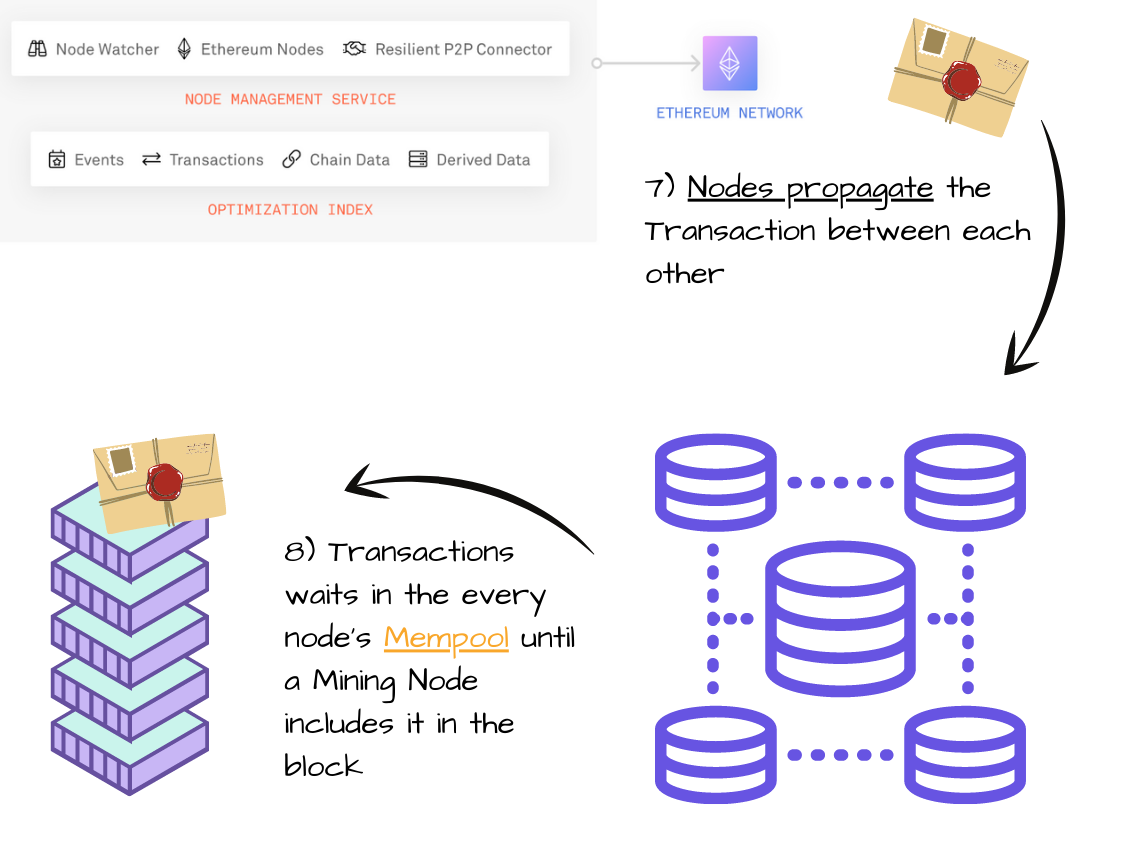
\includegraphics[width=\textwidth]{infura_propagate.png}}
{Infura nodes propagate the TX to other nodes and miners.}

